\documentclass[12pt,review]{elsarticle}
\usepackage{graphicx}
\usepackage{mathptmx}     
\usepackage{natbib}
\usepackage{amsmath}
\usepackage{sidecap}
\usepackage[margin=.8in]{geometry}

\makeatletter
\newtheorem{thm}{\protect\theoremname}
\newtheorem{fact}[thm]{\protect\factname}
\newtheorem{fdn}{Finding}
\makeatother
\providecommand{\factname}{Fact}
\providecommand{\theoremname}{Theorem}
\providecommand{\keywords}[1]{\textit{Keywords:} #1}
\providecommand{\JEL}[1]{\textit{JEL Classification:} #1}
\usepackage{lineno,hyperref}

%\modulolinenumbers[5]

\journal{Journal of Behavioral and Experimental Economics}

%%%%%%%%%%%%%%%%%%%%%%%
%\bibliographystyle{elsarticle-num}
\bibliographystyle{jebo}      % Herbert Gintis to the rescue!
%%%%%%%%%%%%%%%%%%%%%%%


\begin{document}
%\begin{titlepage}
%\thispagestyle{empty}
\newcommand{\HRule}{\rule{\linewidth}{0.5mm}} % Defines a new command for horizontal lines, change thickness here
	
%------------------------------------------------
%	Headings
%------------------------------------------------
	
{\center

\textsc{\LARGE Title Page}\\[1cm]
{\large\today} % Date, change the \today to a set date if you want to be precise

%------------------------------------------------
%	Title
%------------------------------------------------

\HRule\\[0.4cm]
\huge\bfseries Strategic Reasoning Online: Experiments on the Beauty Contest\\[0.4cm]
\HRule\\[0.4cm]
}

%------------------------------------------------
%	Author(s)
%------------------------------------------------

{\center
\large\textbf{Authors:}\\
}

\noindent
Robin \textsc{Engelhardt},  Center for Information and Bubble Studies, University of Copenhagen, Karen Blixens Plads 8, 2300 Copenhagen S, Denmark, email: robin.engelhardt@gmail.com, tel: +45/26300403, ORCID: 0000-0002-7162-0990 \\

\noindent
Paolo \textsc{Galeazzi}, Center for Information and Bubble Studies, University of Copenhagen, Karen Blixens Plads 8, 2300 Copenhagen S,  email:  pagale87@gmail.com.\\
	
{\center
\large\textbf{Acknowledgements}:\\
}

\noindent
The authors wish to thank Mikkel B. Andersen for help with server infrastructure and devops, and Rosemarie Nagel for providing experimental datafiles. The authors gratefully acknowledge the support provided by The Carlsberg Foundation under grant number CF 15-0212.
	
	% \author{Robin Engelhardt and Paolo Galeazzi\thanks{Engelhardt: Center for Information and Bubble Studies, University of Copenhagen, Karen Blixens Plads 8, robin.engelhardt@gmail.com. Galeazzi: Center for Information and Bubble Studies, University of Copenhagen, Karen Blixens Plads 8, pagale87@gmail.com. Acknowledgements}}

	




%\end{titlepage}


\begin{frontmatter}
\title{The Beauty Contest On Amazon Mechanical Turk: Going Further Into The Field\tnoteref{t1}}
%\tnotetext[t1]{This document is the results of the research project funded by The Carlsberg Foundation under grant number CF 15-0212.}

\author{Robin Engelhardt\corref{cor1}}
\ead{robin.engelhardt@gmail.com}
\author{Paolo Galeazzi}
\ead{pagale87@gmail.com}
\cortext[cor1]{Corresponding author}
\address{Center for Information and Bubble Studies, University of Copenhagen, Karen Blixens Plads 8, 2300 Copenhagen, Denmark}


\begin{abstract}
We examine the process of reasoning among 296 subjects playing the
iterated beauty contest game on Amazon Mechanical Turk (MTurk). Our findings
are substantially different from the behaviors observed in laboratory
and newspaper experiments reported in the literature. In general,
we do not find any strong evidence in favor of higher-order reasoning
in the first round as well as in the following iterations of the game,
which puts into question the presence of any strategic thinking among
the vast majority of subjects on MTurk.
\newline
\keywords{Beauty Contest,  Mechanical Turk,  Iterated best response,  Higher-order reasoning}
\newline
\JEL{C72, C73}
\end{abstract}

%\begin{keyword}
%Beauty Contest \sep  Mechanical Turk \sep  Iterated best response \sep  Higher-order reasoning
%\end{keyword}

\end{frontmatter}

\linenumbers

\section{Introduction\label{sec:Introduction}}
\noindent
The so-called \emph{beauty contest game} has been introduced by \citet{Keynes:1936} to explain how expectations about the beliefs of other agents play a crucial role in financial markets. The label \textquotedblleft beauty contest\textquotedblright{} nowadays encompasses a variety of different experimental games having in common the key role played by the subjects' ability to think about each others thought processes, e.g. their `theory of mind' and depth of strategic reasoning  \citep{NagelEtAl02, CamererHoChong2004, DuffyNagel97, NagelGrosskopf2008, HoCamererWeigelt98, Nagel95, Rapoport06}. The most well-known example, due to \citet{Moulin86}, is the following: each player has to choose a number in the interval {[}0, 100{]}; the players who are the closest to $2/3$ of the average of all chosen numbers evenly split a fixed positive monetary amount. The only equilibrium of this game is when all players choose the lowest number, zero. However,
choosing zero may not win the game: if for instance there are more than two players in the game, and a player believes that all other players are going to pick a number sufficiently greater than zero, then zero is not a best response.

The beauty contest has been extensively tested in experiments to study the players' depth of strategic reasoning -- i.e., the number of steps in an unobservable process of reasoning about each other intended to explain the behavior of agents in interactive decision making \citep{NagelEtAl02, CamererHoChong2004, NagelGrosskopf2008, HoCamererWeigelt98, Nagel95}. Loosely, the idea is that the higher the level in the depth of reasoning, the lower the chosen number will be \citep{BURNHAMetAl2009-BCgame}. A player with depth of reasoning of level zero simply chooses a random
or salient number between 0 and 100 in the first round. Two different solution concepts have been proposed to capture the higher-order reasoning of players. According to the first, called \emph{degenerate}\footnote{The term ``degenerate'' comes form the assumption that each agent assigns probability 1 to the other players being of exactly one reasoning level lower than herself.} \emph{iterated best response reasoning} (IBRd) and used for instance in \citet{Nagel95} and \citet{NagelEtAl02}, a player of level one is supposed to best respond to the belief that his or her opponents are of level zero. Therefore, a player of level one would choose (a number close to) $50\cdot2/3=33.3$, which is the best response to the belief that the other players choose at random from a symmetric distribution around 50. By iterating the same reasoning once more, a player of level two would choose (a number close to) $50\cdot(2/3)^{2}=22.2$. By repeating this reasoning infinitely many times, a player with infinite depth chooses the minimum, zero. 

An alternative solution concept for capturing the higher-order reasoning of players, used e.g. in \citet{HoCamererWeigelt98}, is the iterated elimination of dominated strategies. A player of level one accordingly chooses only numbers from the interval $[0,2/3\cdot100]$, because any number in the interval $(2/3\cdot100,100]$ is dominated by $2/3\cdot100=66.6$.
By iterating the same reasoning, a player of level two, chooses only numbers in the interval $[0,(2/3)^{2}\cdot100]$, and the process converges again to zero as the levels of depth go to infinity. Infinite iterations of either solution concept thus lead to the sole equilibrium of the game.

The bulk of classic experiments on the beauty contest have been carried out as lab experiments with small- and medium-sized groups of university students (e.g. \citet{Nagel95, HoCamererWeigelt98}, see also \citet{CamererHoChong2004} and \citet{Nagel08Chapter} for an overview), or as single-shot large-scale newspaper contests \citep{bosch1997juego, schou2005gaet, selten1998zahlenwahlspiel, Thaler1997competition}. These experiments report findings of higher-order reasoning and classify most subjects between level one and level two of depth of reasoning \citep{NagelEtAl02, DuffyNagel97, HoCamererWeigelt98, Nagel95, Rapoport06, selten1998zahlenwahlspiel}. A high number of guesses in the proximity of the numbers 33 and 22 in the first round are found by \citet{Nagel95, selten1998zahlenwahlspiel} and interpreted as revealing the presence of IBRd as well as of one or two levels of higher-order reasoning by the majority of subjects. This finding is later confirmed by a survey of the results from laboratory, classroom, and also in the newspaper experiments.

%The paper is organized as follows. After describing our experiments in Section~\ref{sec:Method}, the findings are analyzed in detail in Section~\ref{sec:Results}, which is divided into two parts corresponding to the first round (Subsection~\ref{subsec:Static:-First-Round}) and to subsequent rounds (Subsection~\ref{subsec:Dynamic:-Subsequent-Rounds}). Section~\ref{sec:Discussion} discusses our findings in the light of previous work, and Section~\ref{sec:Conclusion} concludes. 

\section{Method\label{sec:Method}}
\noindent
Testing whether the same behavioral pattern can be found in subject pools very different from students in classrooms and experimental labs, as well as from self-selected readerships in high-profile newspapers, we designed a set of iterated beauty contest experiments on Amazon Mechanical Turk (MTurk), an online labor market and crowd sourcing platform which has been shown to be reliable, replicable, and significantly more diverse than typical American college samples \citep{BuhrmesterEtAl2011,CrumpEtAl13,HortonEtAl2011,Rand2012}. We conjectured that in contrast to students, subjects on MTurk supposedly have little or no prior knowledge of these types of reasoning games, and that the limited time available for them to think about their guess also would set them apart from typical newspaper readers who have participated in beauty contests previously. 

A total of 296 participants were recruited from MTurk and randomly split into 50 two-player groups, 23 four-player groups and 13 eight-player groups. After the groups were formed, and informed consent was given, players were introduced to the game in the following way:

\begin{quote}
Instructions: You are in a group of 2 {[}4 or 8, respectively{]} players.
In each round players will be asked to choose a number between 0 and
100. The winner will be the player whose number is closest to $2/3$
of the average of all chosen numbers. The game has 8 rounds. Payoffs:
Each player will receive a participation fee of \$2 after finishing
the game. In addition, the winner in each round will get a bonus of
\$0.25 {[}\$0.5 or \$1, respectively{]}. If there is more than one
winner the bonus is split. Examples: if you choose 30 as the number
closest to $2/3$ of the average and win the round, you will receive
\$0.25 {[}\$0.5 or \$1, respectively{]}. If you and another player
guess 20 and win, you will win half of the bonus.
\end{quote}

The payoff structure ensures that players receive on average the same bonus across different group sizes and are unlikely to quit the game prematurely, because the overall bonus after eight rounds could potentially become substantially larger than the flat participation fee of \$2. After each round, each player's guess was recorded, and players were shown the winning guess, the full list of previous guesses by all players, the averages in all previous rounds, as well as the $2/3$ of those averages.\footnote{Players could only select integers between 0 and 100 in our MTurk experiments. While discrete action spaces may make some new equilibria arise, the only new equilibrium in our case is a profile of ones in the 8-player beauty contest. In general, when the number of players is not large, all new equilibria are profiles of low numbers, which does not affect the initial steps of the reasoning processes described in Section~\ref{sec:Introduction}. See \citet{SeelTsakas17} for more details.} After round 8 players were thanked and asked about the strategy they used when playing the game, which provided valuable information on the players\textquoteright{} decision making process. No player was allowed to play the game twice.\footnote{See supplementary information for more details about the experimental design.}

\section{Results\label{sec:Results}}
\noindent
Beauty contests have often been designed as one-shot experiments, which corresponds to only looking at the results in round 1 of our experiments. Like in the classic papers on this topic (e.g. \citet{Nagel95, HoCamererWeigelt98}), we analyze the results from the first round and from the subsequent rounds separately.

\subsection{Static: First Round\label{subsec:Static:-First-Round}}
\noindent
Figure~\ref{fig:1} shows the distributions of guesses from a selected sample of previous experiments on the beauty contest also analyzed in \citet{NagelEtAl02}.\footnote{We only show distributions from previous experiments, where we could get hold of the complete data set.} The lowest means are found among theorists, in the internet newsgroup experiment, and in the newspaper experiments. Specifically, the newspaper experiments were done in the magazine \textit{Spektrum der Wissenschaft} \cite{selten1998zahlenwahlspiel} (with a mean of 22.1), in the \textit{Financial Times} \cite{Thaler1997competition} (mean 18.9) and in the Spanish newspaper \textit{Expansión} \cite{NagelEtAl02} (mean = 25.5). Another large scale experiment with 19,196 readers of the Danish daily newspaper \textit{Politiken} reported a mean of 32.4 \cite{schou2005gaet} (not shown here). The presence of spikes in the vicinity of 22.2 and 33.3 in the majority of experiments shown in Figure~\ref{fig:1} supports the conclusions that subjects can be described as performing one or two iterations of best response reasoning and that the IBRd model may provide a good description of how people behave and reason about each other in the beauty contest. 

\begin{figure}
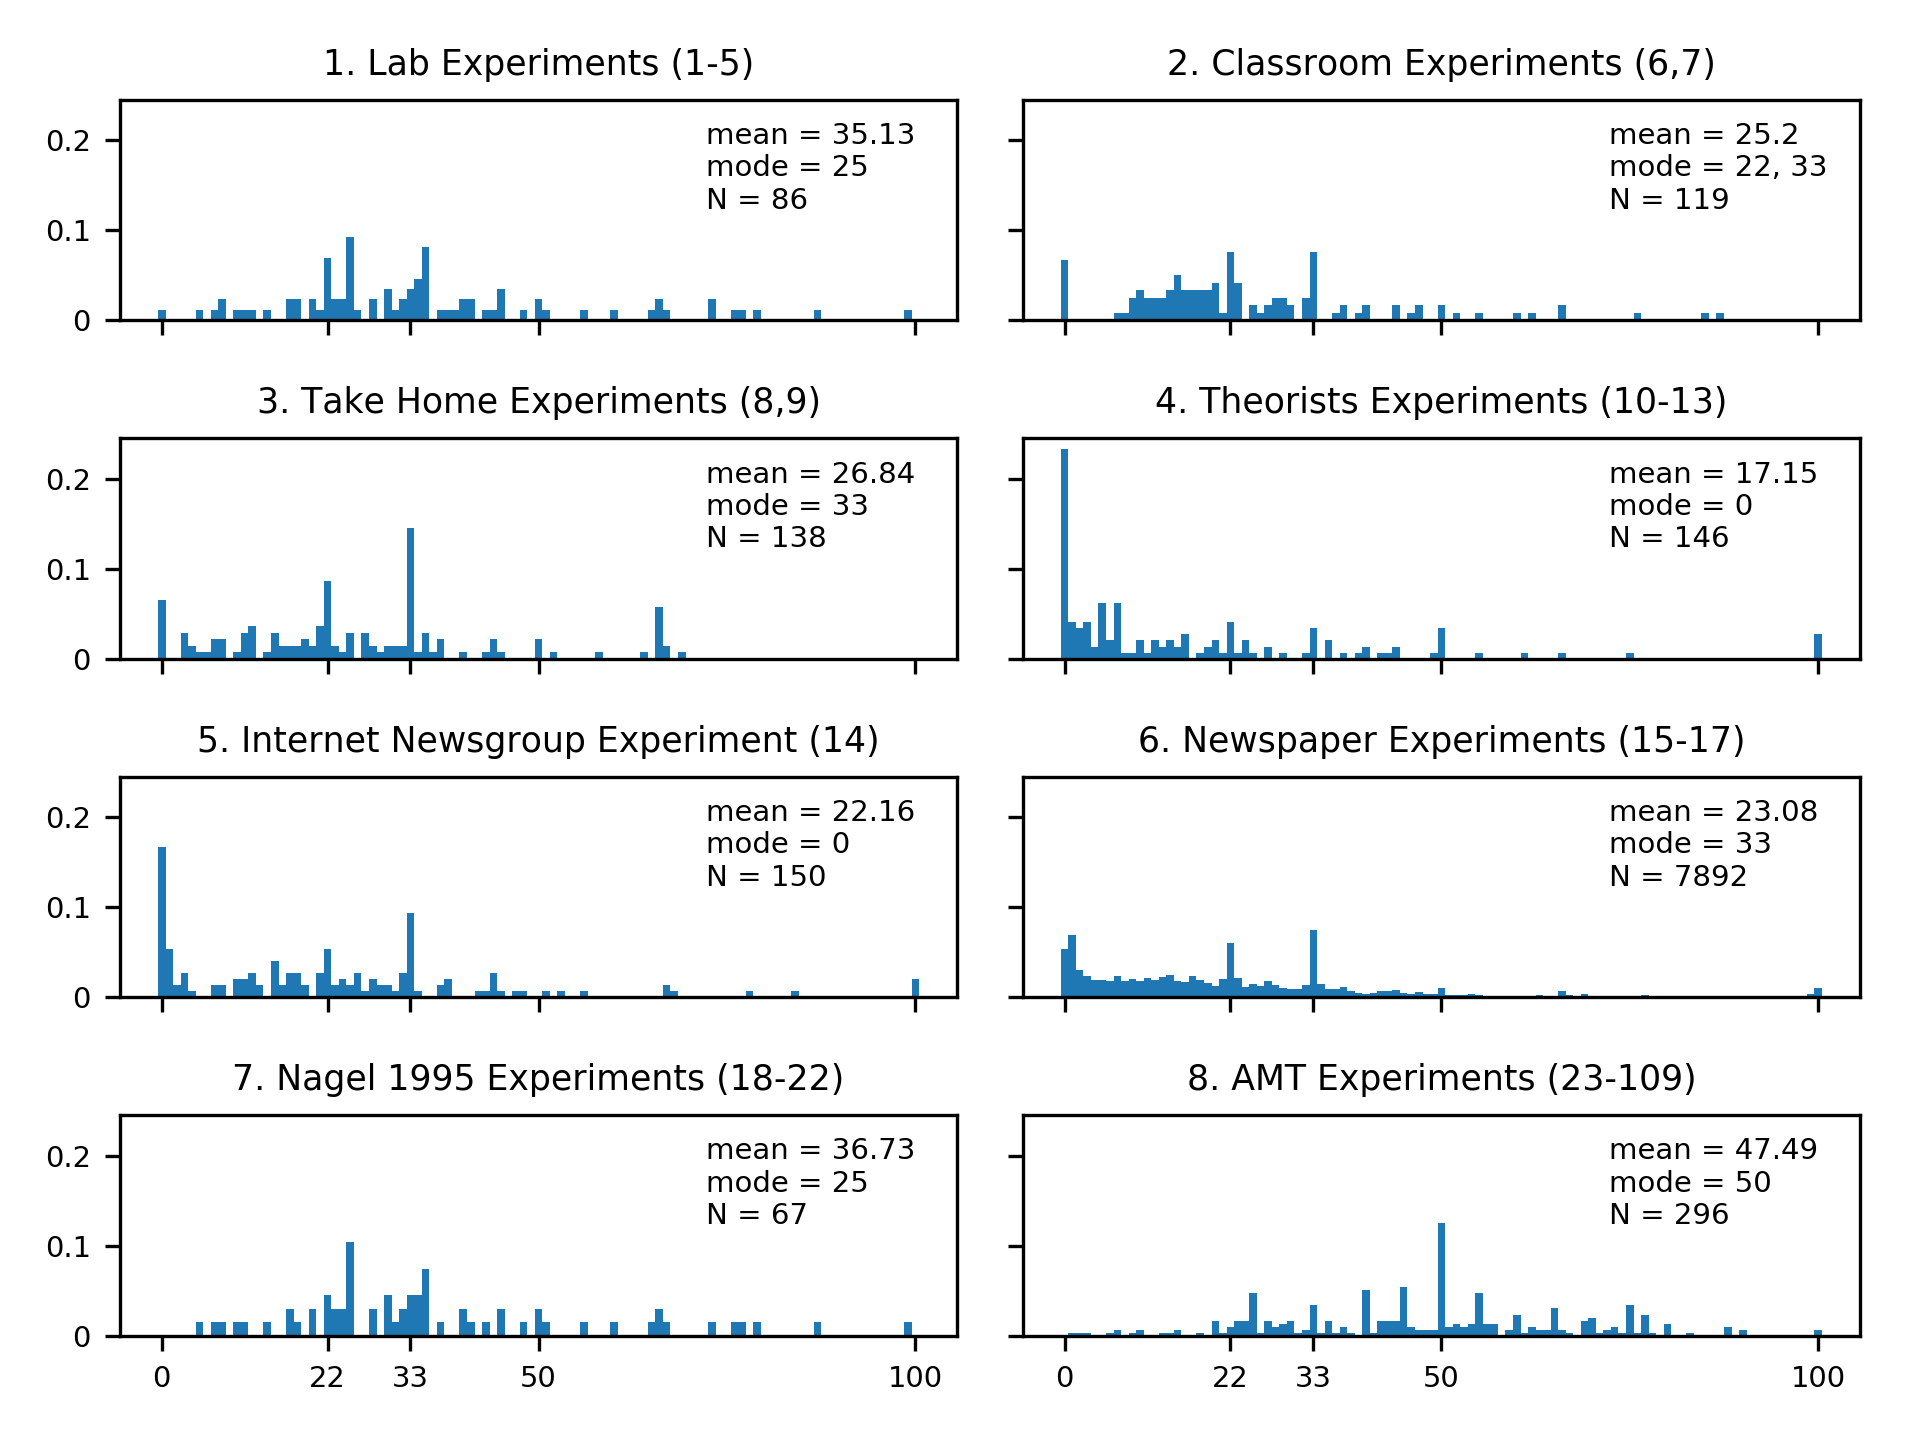
\includegraphics[width=1\textwidth]{../plots/fig1.pdf}\caption{The first six subplots show the distributions of guesses from various ``one shot'' lab and newspaper experiments as analyzed by \citet{NagelEtAl02, Thaler1997competition, selten1998zahlenwahlspiel} and \citet{bosch1997juego}. The bottom left subplot depicts the distribution of guesses in the first round in the experiments by \citet{Nagel95}, while the bottom right subplot shows the distribution of the results we collected from the first round on MTurk.}
\label{fig:1}
\end{figure}

Our findings from MTurk, shown in the bottom right graph of Figure~\ref{fig:1}, tell a different story. First of all, while the mass of all other distributions is concentrated on the left half of the interval {[}0,100{]}, the distribution of the data from MTurk is close to normal ($p=0.047$, Shapiro-Wilk test) with mode 50 and mean 47.49, and has mass concentrated around the center of the interval and spreading away symmetrically in both directions. Moreover, when we consider the three different treatments individually, all still have mean above 45 (50.99 for 2-player groups, 45.42 for 4-player groups and 45.96 for 8-player groups), and the mode is 50 for each treatment too, overall indicating a propensity towards a middle number in the first round. Second, unlike the other seven distributions in Figure~\ref{fig:1}, the one from MTurk has no notable spike either around 33.33 or around 22.22. A major spike at 50 is instead present, which corresponds to the modal choice, while lower spikes appear more or less symmetrically on both sides of it. We can therefore state the following:

\begin{fdn}
No spikes confirming the effect of some iterations of IBRd reasoning are found in our MTurk-experiments.
\end{fdn}

The IBRd model assumes that the iteration process starts from 50, as detailed in Section~\ref{sec:Introduction}. Such a starting point may be interpreted as the expectation from randomly choosing according to a symmetric distribution around 50, or alternatively as the choice of a salient number \`{a} la Schelling \citep{sch60}. The distribution of choices on MTurk is compatible with both these hypotheses: given the marked central spike, we can exclude that the symmetric distribution is uniform, hence supporting some sort of salience in the number 50. A second conclusion can then be drawn from our experiments: 

\begin{fdn}
The behavior observed in MTurk experiments is compatible with players choosing at random from a symmetric distribution with mean 50, possibly viewed as a salient number. Relative to the IBRd model, this can be interpreted as a population of 0-level players, choosing numbers at random or by simple salience, without any higher-order reasoning.
\end{fdn}

\subsection{Dynamic: Subsequent Rounds\label{subsec:Dynamic:-Subsequent-Rounds}}
\noindent
Clear evidence in favor of higher-order reasoning is not found in subsequent rounds either. Figure~\ref{fig:means} shows the least square means of each of the eight rounds played on MTurk with groups of size 2, 4, and 8, respectively. For comparison we plot the results of the experiments by \citet{Nagel95}, by \citet{Kamm2008unter} as reported in \cite{diekmann2009rational}, by \citet{weber2003learning}, and by \citet{buhren2010chess}, all shown without colors\footnote{Having only summary data of those experiments, we can not fit a regression model and report on their confidence intervals. For a least square fit on all rounds of the MTurk experiment, see the appendix which also contains histograms of all MTurk data partitioned into group sizes and rounds.}. 

\begin{figure}
\includegraphics[width=1\textwidth]{../plots/fig3_new.pdf}
\caption{Means for iterated beauty contest experiments with various number of rounds. Least square fits of MTurk-experiments with group sizes 2, 4 and 8 are shown in colors. Results from lab experiments with students by \citet{Nagel95} (N95), \citet{Kamm2008unter} (KD08), \citet{weber2003learning} (W03), and with chess players by \citet{buhren2010chess} (BF10) are shown without colors. N is the total number of participants and n is the group size. Note that the linear regression model for the MTurk-experiments is only fitted to the first 4 rounds, hence the regression lines and $95\%$ confidence intervals are only plotted for rounds 1-4. A quadratic terms is necessary to extrapolate these (especially for the groups of 8's) to round 8 (see appendix).}
\label{fig:means}
\end{figure}

Clearly all MTurk-experiments have significantly higher means than the other experiments reported here. In addition, MTurk-experiments with two players have significantly higher means than MTurk-experiments with four and eight players, indicating that people may behave differently when playing against only one opponent. As already noticed in \citet{HoCamererWeigelt98}, this is puzzling in that the smaller the group, the larger the effect of individual guesses on the mean. Two-person beauty contests are in fact isomorphic to the game \textquotedblleft whoever chooses the smaller number wins\textquotedblright : while one is not guaranteed to win when choosing zero in the 4- or 8-player beauty contest, guessing zero is weakly dominant and ensures at least a tie in the 2-player game. In our 50 experiments with groups of two players, there was no participant who chose zero in the first round. After 8 rounds, zero was chosen 3 times in total (out of 800 guesses). This is significantly lower than what was found previously by \citet{NagelGrosskopf2008}, where about 10\% of undergraduates in economics guessed zero in the one-shot version of the 2-player game.

\subsubsection{Learning}
\noindent
The decreasing means in Figure~\ref{fig:means} may be interpreted as a sign of learning. The rates of learning, however, differ between experiments. To compare rates of learning directly, we extract the slope coefficients ($\beta$-estimates) along with their standard deviations from the linear regression model of the MTurk-experiments and calculate $95\%$ confidence intervals for each group. Discarding any uncertainties in the other studies, we simply calculate their rates of learning as the slopes of the ``optimal'' straight lines through the reported round averages. 

\begin{SCtable}
\begin{tabular}{lcccc}
\hline
Experiment	& n & N 	& $\beta$ & $95\%$ CI \\
\hline
MTurk	&	2			&	100	&	-3.32 & 	(-4.26, -2.38)	\\
	   	&	4			&	92 	&	-5.71 &	(-6.67, -4.73)	\\
	   	&	8			&	104	&	-6.34 &	(-7.26, -5.42)	\\
BF10	&	13-897		&	26	&	-6.45 &\\
W03  	& \{8,8,10\} 	&	26	&	-6.49 &\\
KD08	& 14 			& 14 	&	-6.83 &\\
	   	& 50 			& 50 	&	-7.97 &\\
	   	& 188 			& 188 	&	-5.54 &\\
N95		&\{15,16,18,18\}& 67 	&	-8.97 &\\
\hline
\end{tabular}
\caption{Rates of learning in iterated p-beauty contest experiments with $p=2/3$. n = group size; N = number of subjects; $\beta$ = slope coefficient of means from round 1 to round 4 (for BF10, $\beta$ is calculated from round 1 to round 2 only).}
\label{table:1}
\end{SCtable}

Comparing the $\beta$'s in Table \ref{table:1}, we find that only `KD08.50` and `N95` are quite different from all MTurk groups. The rest are within the limits of the MTurk groups of 4 or 8. The `kd08.50` experiment is just beyond the confidence bounds, and even though the reported $\beta$'s from the other studies do not have confidence bounds, some uncertainty is to be expected here. Taking the MTurk standard deviations as a proxy, the intervals are roughly $\approx\beta\pm1$, hence the `kd08.50` can be reasonably expected to overlap the confidence interval of $\beta_{MTurk.8}$. Hence, we can conclude that the rate of learning is quite similar for most studies, and coincide with the findings of MTurk-groups of 4 and 8 players. Only the MTurk-groups consisting of 2 players are significantly different from everything else, including MTurk groups with 4 and 8 players. This indicates a significantly different kind of behavior in beauty contests with two players.

Higher learning rates are sometimes associated with larger group sizes (\citet{HoCamererWeigelt98}, p. 958), but the similarity in the learning rates of 4 and 8 player MTurk groups, and the learning rates in the other small-group experiments in `BF10', `W03', and `KD08' (see Table \ref{table:1}) are counterexamples to that association. Our MTurk-experiments also seem to be at odds with the hypothesis that larger groups choose higher numbers at the start (see \citet{HoCamererWeigelt98}, p. 958). What holds true though, is that the 2-person beauty contest constitutes a puzzling case in which players not only lack the strategic sophistication to understand the great power in their hands, but even display a tendency towards higher guesses than in groups with more than two players. A possible explanation, also suggested by \citet{NagelGrosskopf2008}, see also \citet{chou2009control}, may be based on a cognitive misconception of the game: players might aim to be as close as possible to the $2/3$ of the mean rather than to be clos\emph{er} than the opponent to the $2/3$ of the mean. We can thus state the following:

\begin{fdn}
The means of beauty contests on MTurk are significantly higher than the means reported in previous classroom, lab- and newspaper experiment. However, by looking at the slope coefficients of the various iterated beauty contests, we find comparable rates of learning across all experiments, except for beauty contests with two-person groups, which are significantly different from all other group sizes.
\end{fdn}

It is noticeable that simple directional learning seems to be falsified by our MTurk experiments. Figure \ref{fig:4} pictures the distribution of the number of times a player chooses a number greater than the target of the previous round, i.e., greater than $2/3$ of the previous mean. Experiments on MTurk, on the right, show that less than 2\% of players never guess higher than the target of the previous round, while the vast majority (more than 80\%) does that at least three times, and about 50\% does it five times or more.

\begin{figure}
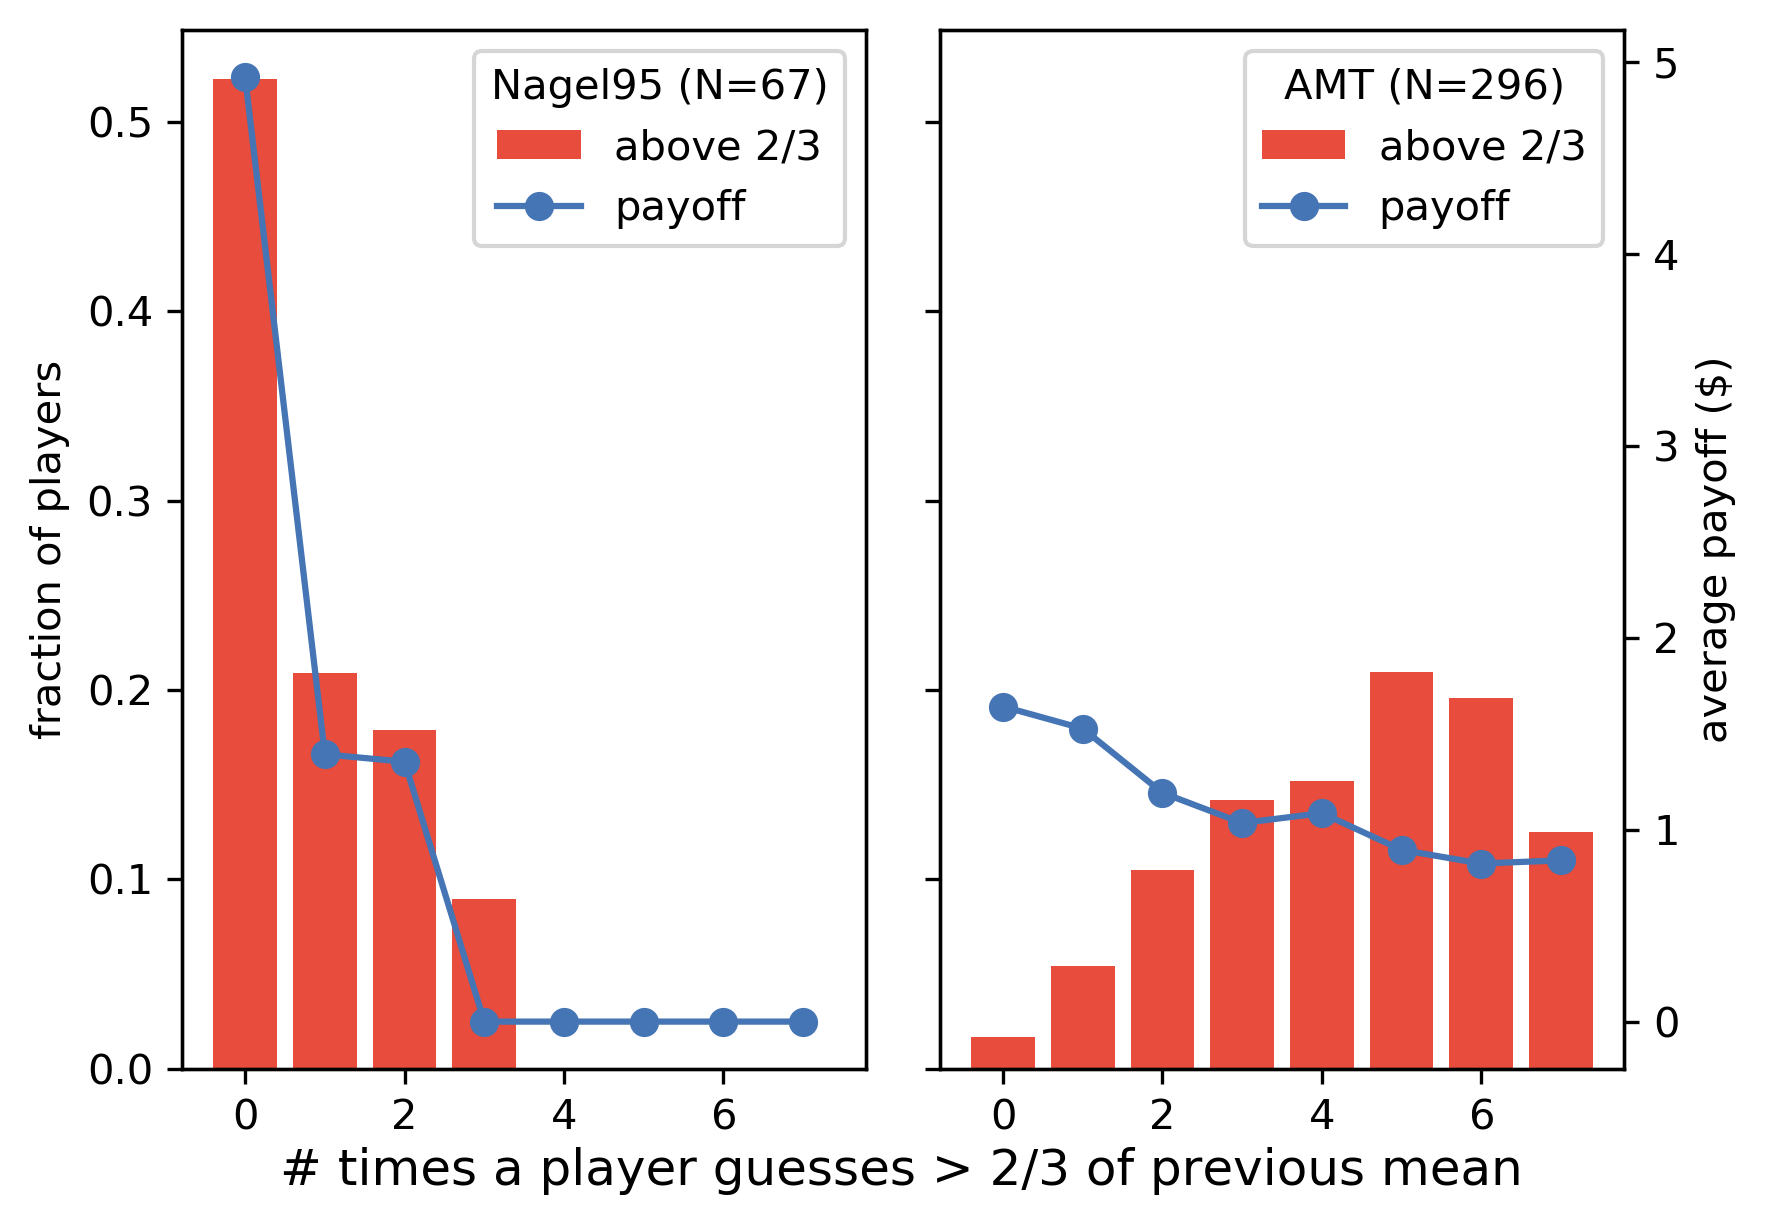
\includegraphics[width=1\textwidth]{../plots/fig4.pdf}
\caption{Bar chart of the number of times a player chooses a number greater than $2/3$ of the mean of the previous round. In the lab experiments by \citet{Nagel95} (left) 52\% of the players never go above $2/3$
of the previous mean, and only about 25\% do that more than once. In the MTurk experiments (right) less than 2\% of players never go above $2/3$ of the previous mean, while 53\% of players go above $2/3$ of the previous mean more than four times. Average payoffs for these player types (blue) are shown for comparison only.}
\label{fig:4}
\end{figure}

The distribution on the left, corresponding to the lab experiments by \citet{Nagel95}, depicts players of a different kind: more than 50\% of players never go higher than the target of the previous round, while only about 25\% do that more than once. Importantly, let us stress that both in the lab experiments on the left and in the experiments on MTurk, at the end of each round players were told the two-thirds of the mean of that round, as well as all chosen numbers. While the players in \citet{Nagel95} seem to learn that the target decreases and adapt to this, players on MTurk cannot be viewed as adapting to a decreasing target: most of the times they pick numbers higher than $2/3$ of the mean of the previous round, even while observing a decreasing sequence of means and targets.

From the assumption that, in subsequent repetitions, a player of level zero chooses at random according to a symmetric distribution around the previous mean (or the previous target), it follows that a player of level one would never guess higher than the previous target, and higher levels of reasoning imply even lower guesses. Hence, the combination of some iterations of IBRd with an adaptation process taking the two-thirds of the mean of the previous round as reference point for the next round is incompatible with the behavior observed on MTurk. 

\section{Discussion\label{sec:Discussion}}
\noindent
In light of the results above, one may want to reassess the role played by subject pools with differing demographical compositions playing the game in distinct settings and contexts. Participants in lab and classroom experiments are most often university students, sometimes even graduate or PhD students in economics, and hence cannot be considered as typical exemplars of the population. This causes issues about the sociodemographic representativeness of such samples: how generalizable are the results from lab and classroom experiments? 

The same question can be asked about newspaper experiments. On one hand newspaper beauty contests reach a broader and more diverse population, but there is no control of the sociodemographic characteristics of readers, who in the end decide to participate and send in a guess. A first attempt at this discussion was made by \citet{NagelEtAl02}, who argue that newspaper experiments should be considered field experiments, and that the similar results between newspaper experiments and lab/classroom experiments shown in figure \ref{fig:1} warrant a \textquotedblleft parallelism\textquotedblright {} between the lab and the field (\cite{NagelEtAl02}, page 1697). In other words: labs and classroom experiments are close to the field as well. The sizeable differences to our result, though, would lead to another conclusion: The ``field'' is not very well captured by neither students nor newspaper readers. 

But what about MTurk? Is the MTurk subject pool more representative of the population at large, or is it just very different from other subject pools such as undergraduate students? This question has been discussed extensively in the literature \cite{BuhrmesterEtAl2011, chandler2015using, CrumpEtAl13, hauser2018common, HortonEtAl2011,  landers2015inconvenient, paolacci2014inside, Rand2012, stewart2015average}, and while there are good arguments for saying that no survey platform is truly representative of the whole (global) population, most researchers agree that MTurk compares well with (american) undergraduate samples in diverse fields such as cognitive psychology \cite{CrumpEtAl13}, social psychology \cite{klein2014investigating}, judgment and decision-making \cite{paolacci2010running}, and economics \cite{amir2012economic}, and recommend that reviewers and editors should consider accepting behavioral experiments done on MTurk as a valid methodology \cite{CrumpEtAl13, hauser2018common}.

What about concerns about the quality of our data collected from MTurk? There may be concerns about the sufficiency of monetary incentives, about the lack of attention and/or cognitive ability and effort. Addressing the first of those, our average payoff was approximately \$15 per hour, which is considered generous according to MTurk guidelines and certainly above the estimated average of \$6 per hour when excluding unsubmitted and rejected work \citep{HaraEtAl18}. In addition, the belief that data quality depends on the (relative) size of the bonus compared to the participation fee is contradicted by \citet{amir2012economic}, who showed that results of standard economic games with very low bonuses on MTurk are comparable to those of corresponding lab experiments with higher bonuses, thus alleviating concerns about the validity of economic game experiments conducted on MTurk. 

With regard to possible concerns about insufficient cognitive ability and/or effort among MTurk subjects, we can only suggest that for economic games to be representative of the real world, they should not necessarily require subjects to be experts or be trained in any particular way. If the aim were to test the cognitive acumen of economists and mathematically talented people only, MTurk may not be the best place for such experiments. If, however, the purpose is to investigate normal people's use of higher-order reasoning in online settings, MTurk may be a good place to start. 

As discussed by \citet{chou2009control}, the apparent lack of strategic thinking among the majority of subjects in the two player version of the game may be due to the fact that the beauty contest is an unfamiliar type of game in which subjects lack understanding of the relationships between possible choices, outcomes and payoffs. This lack of understanding of the game form may also be present in groups with four and eight players. Online platforms like Amazon Mechanical Turk, where subjects have no prior knowledge, limited time and little patience, may amplify such misconceptions.

To conclude the discussion, the differences between our results and previous results from newspaper, lab, and classroom experiments are most likely due to the disparities between subject pools. We therefore conjecture that the similarity between many of the previous beauty contests may be due to the similarity between their subject pools. Although it is true that the design of the newspaper experiments entails a loss of control on the sample, it does not necessarily follow that the newspaper samples are very different from samples used in lab experiments. Having chosen markedly economic-oriented newspapers might have brought the experimenters not very far into the field. Further lab, field, and MTurk experiments that control for some of the factors discussed above should be able to put more light on the differences we have found.

\section{Conclusion\label{sec:Conclusion}}
\noindent
Beauty contest games on Amazon Mechanical Turk exhibit different behavior from what has been found previously in university laboratories, in classrooms experiments, as well as in high-profile national newspapers. In the one-shot version of the game, the observed behavior on MTurk is compatible with subjects choosing at random from a symmetric distribution with mean 50. Relative to the degenerate iterated best response (IBRd) model, this can be interpreted as a population of 0-level players, choosing numbers at random or by simple salience without any `spikes' that may indicate higher-order reasoning. 

In the iterated version of the beauty contest, groups on MTurk have significantly higher means than what has been found elsewhere. However, by looking at the slope coefficients of the means, we find lower but comparable rates of learning across all experiments, except for the two-person groups, which have a significantly lower learning rate than all other group sizes. Compared to the experiments by \citet{Nagel95}, which have the highest learning rates, we find that subjects on MTurk adapt less linearly to the decreasing target of $2/3$ of the mean, which may be the main reason for the relatively low learning rates found on MTurk.

The differences between our results and previous results from newspaper, lab, and classroom experiments are most likely due to difference in the subject pools and differences in the experimental platform. Controlling for some of these factors in future experiments may improve our understanding of the apparent context dependencies of the beauty contest game.

\section{Acknowledgments}
\noindent
The experiments were implemented by Robin Engelhardt. Server infrastructure and devops was handled by Mikkel Birkegaard Andersen. The authors wish to thank Jacob Stærk-Østergaard for help with the statistical analysis and Vincent F. Hendricks for enabling the project. We are deeply grateful to Prof. Rosemarie Nagel for sharing her data with us. This research was approved by the Institutional Review Board at the University of Copenhagen and included informed consent by all participants in the study. The authors gratefully acknowledge the support provided by The Carlsberg Foundation under grant number CF 15-0212.

\bibliography{gor}  
\newpage
\appendix
\setcounter{page}{1}
\title{Supplementary Material for the article `The Beauty Contest On Amazon Mechanical Turk: Going Further Into The Field'}
%\maketitle

\section{Materials and Method}
\noindent
Amazon Mechanical Turk (MTurk) is an online labor market and crowdsourcing platform, which is increasingly being used for social and economic experiments in order to investigate the real time interactions of small to medium sized groups. MTurk has repeatedly been shown to meet or exceed the standards set by data collection methods using other means \citep{berinsky_huber_lenz_2012, BuhrmesterEtAl18}. The platform has a large participant pool (called participants), various demographic and quality selection options for researchers, and provides an integrated participant compensation system.

\section{Experimental Design}
\noindent
After participants accept our ‘HIT’ (‘human intelligence task’), they have to provide informed consent, see Figure \ref{Fig S1}. Then they wait until there are enough participants who have accepted the HIT to form random groups (grouped by arrival) of size 2, 4 or 8, respectively, depending on the treatment condition. When group has been formed, instructions are displayed for 90 seconds, see Figure \ref{Fig S2}. After pressing NEXT, participants see a page where they have to enter into a form field an integer number between 0 and 100. When all participants in a group have done so, a result page is displayed, see Figure \ref{Fig S3}, where they can see their own guess, the guesses of the other players, the average and the 2/3 of the average as well as information about whether they have won a bonus in the current found and what their total payoff is for the time being. After this, the previous steps are repeated for a total of 8 rounds. Every time participants enter a new number, they can see a list of the 2/3 of the average of the previous rounds as shown in Figure \ref{Fig S4}. participants have 90 seconds to think about a number. After eight rounds, participants are required to give feedback by answering the question: ‘What strategy did you use while playing this game?’, after which they are thanked for their participation.

\begin{figure}
\includegraphics[width=1\textwidth]{../images/FigA1.png}\caption{Screen dump of the consent page shown to all participants.}
\label{Fig S1}
\end{figure}

\begin{figure}
\includegraphics[width=1\textwidth]{../images/FigA2.png}\caption{Screen dump of an instruction page for a game with four players.}
\label{Fig S2}
\end{figure}

\begin{figure}
\includegraphics[width=1\textwidth]{../images/FigA3.png}\caption{Screen dump of a result page from a game with four players.}
\label{Fig S3}
\end{figure}

\begin{figure}
\includegraphics[width=1\textwidth]{../images/FigA4.png}\caption{Screen dump of a choice page from a game with four players.}
\label{Fig S4}
\end{figure}

\section{MTurk Setting}
\noindent
When working with MTurk it is important to consider the right settings in order to get the best data quality possible \citep{ChandlerShapiro16}. Fair wage, attrition rates, removal of duplicate participants and informative feedback are some of the most important issues to address.

Average wage for participants in our experiments was approximately \$15 per hour, which is considered generous according to MTurk guidelines and certainly above the estimated average of \$6 per hour when excluding unsubmitted and rejected work \citep{HaraEtAl18}. 

Quitting a study before completing it is prevalent on MTurk, and varies systemically across experimental conditions. Our overall attrition rate was 24\%, which is considered normal \citep{ZhouFishbach16}. The main reason, we believe, was either a player not being able to enter a number within the allotted time, or – more likely – due to a player not bothering to wait for the others to make their guess and therefore quitting prematurely. This was very detrimental for the rest of the group and for the experiment as such, because it meant that the rest of the group would continue the game with one player less, making the whole process much slower and skewing the results. If somebody had quit, we still let the other players finish their game and paid them for their efforts, but we decided to remove those groups from the data analysis. Out of a total of 114 initial groups, 27 groups were thus removed from the final data set, giving an overall attrition rate of 24\%.

All participants automatically received a unique qualification when accepting a HIT, ensuring that they could not play the game twice. In addition, we set the qualification that participants should have completed at least 50 HIT's and have an accepted HIT rate of 90\% or above. This is slightly below what is considered to be a good cut off point (normally researchers recommend above several hundred completed HIT's and an acceptance rate of 96\%), but we decided to give less experiences players a chance in order not to risk recruiting only those participants who have played this or a similar game before. A 90\% hit rate still ensured that we would get somewhat experienced and qualified participants. During our experiments, participants had also easy access to our email for questions and possible bug reports. 

\section{Code and Software}
\noindent
All experiments are coded in the experimental software oTree 1.4.39 \citep{ChenSchongerWickens16} which is based on Python and Django. The code for the data analysis done is available on Github at https://github.com/gavstrik/BC.

\section{Data Collection and Distribution}
\noindent
After removing defunct groups, we obtained a total of 2368 guesses from 296 unique participants who played the classic iterated beauty contest game in 50 groups of size 2, 23 groups of size 4, and 13 groups of size 8.

\begin{figure}
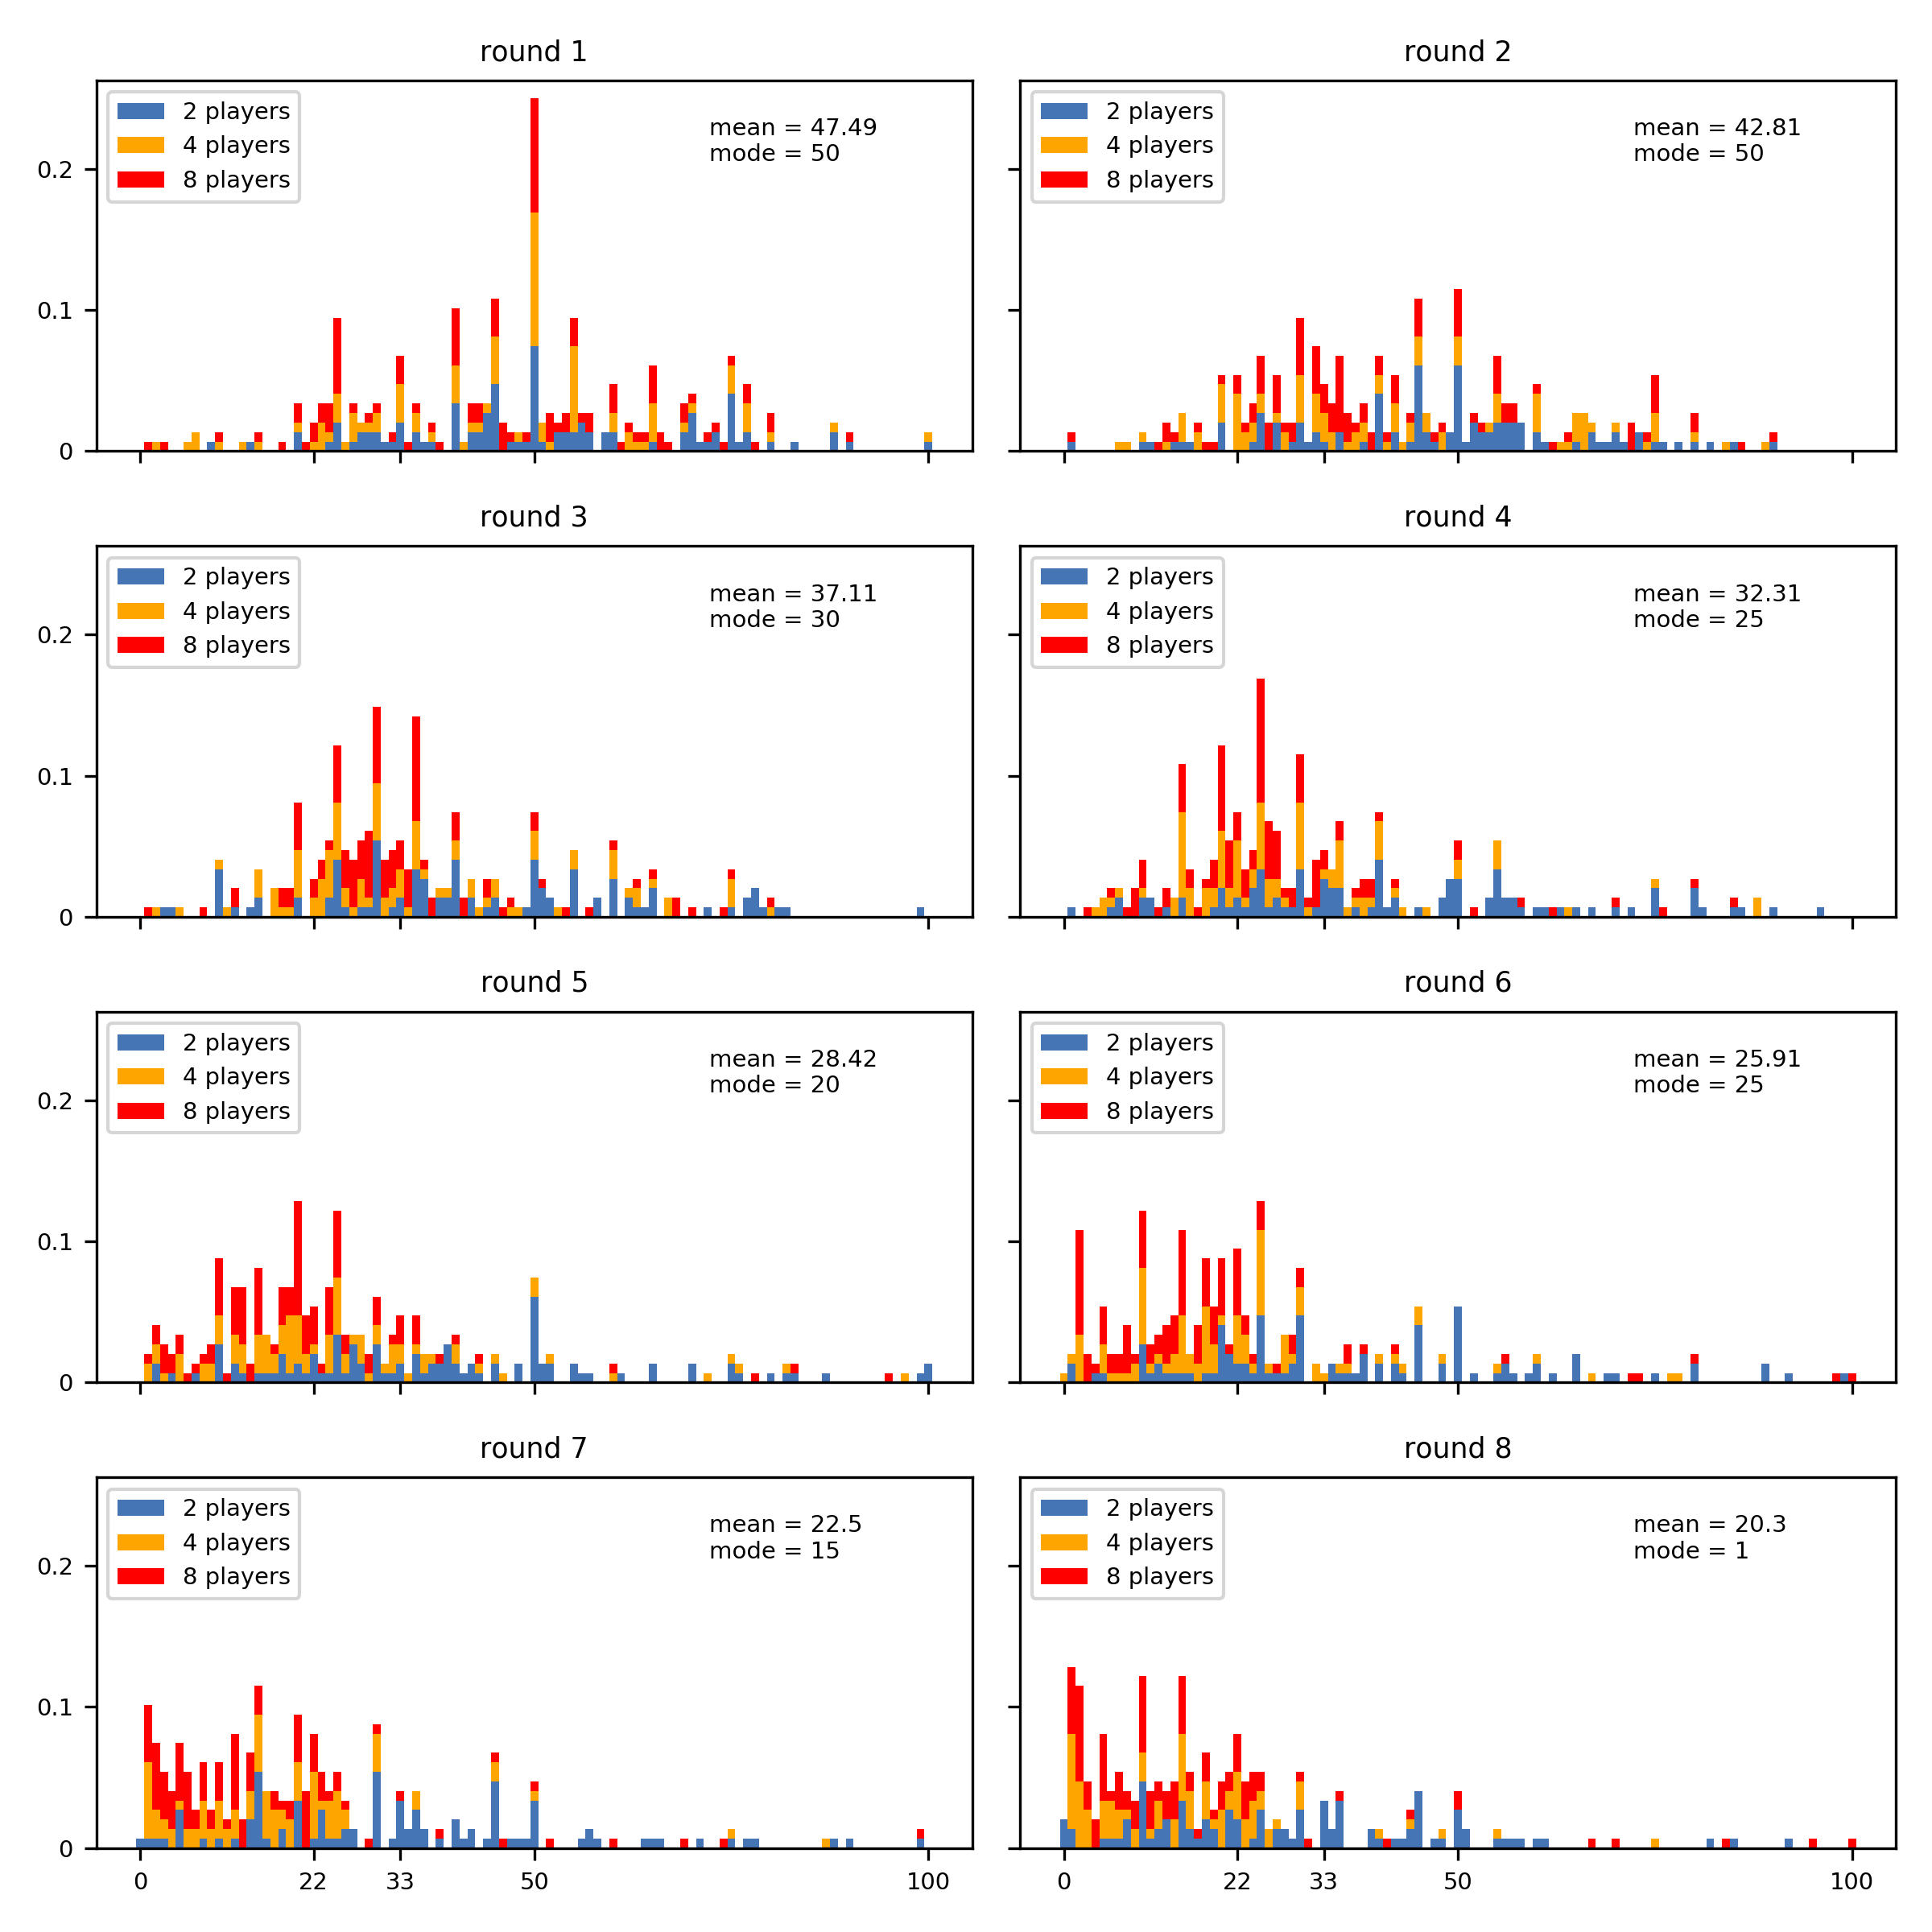
\includegraphics[width=1\textwidth]{../plots/figA5.pdf}\caption{Histograms of guess distributions partitioned into groups and rounds.}
\label{Fig S5}
\end{figure}

Figure \ref{Fig S5} shows the guesses for all eight rounds, partitioned into their respective groups. As can be seen from the histograms, guesses move slowly towards lower numbers in subsequent rounds, with the 2-players groups (in blue) lacking slightly behind the other groups. There are many spikes in the plots, but there is no discernible pattern that would suggest dominant spikes at those positions corresponding to iterated best response strategies (33, 22, etc...).

%\section{Guess Dynamics}
%As noted in figure 4 in the main text, players often choose numbers greater than 2/3 of the mean of the previous round. Less than 2\% of all players on MTurk never go above 2/3 of the previous mean, while 53\% go above this target more than four times. 

%Figure \ref{Fig S6} shows some examples of the up and down movements of individual guesses from one round to the next. It is difficult to interpret this behavior observed in Fig. S6 as simple directional learning. Instead, players seem to try to “talk” with each other with occasional high guesses, and instead of adapting to the new target (explicitly shown as 2/3 of the previous mean), they may adapt to what they think the other players will guess in the next round.
%
%\begin{figure}
%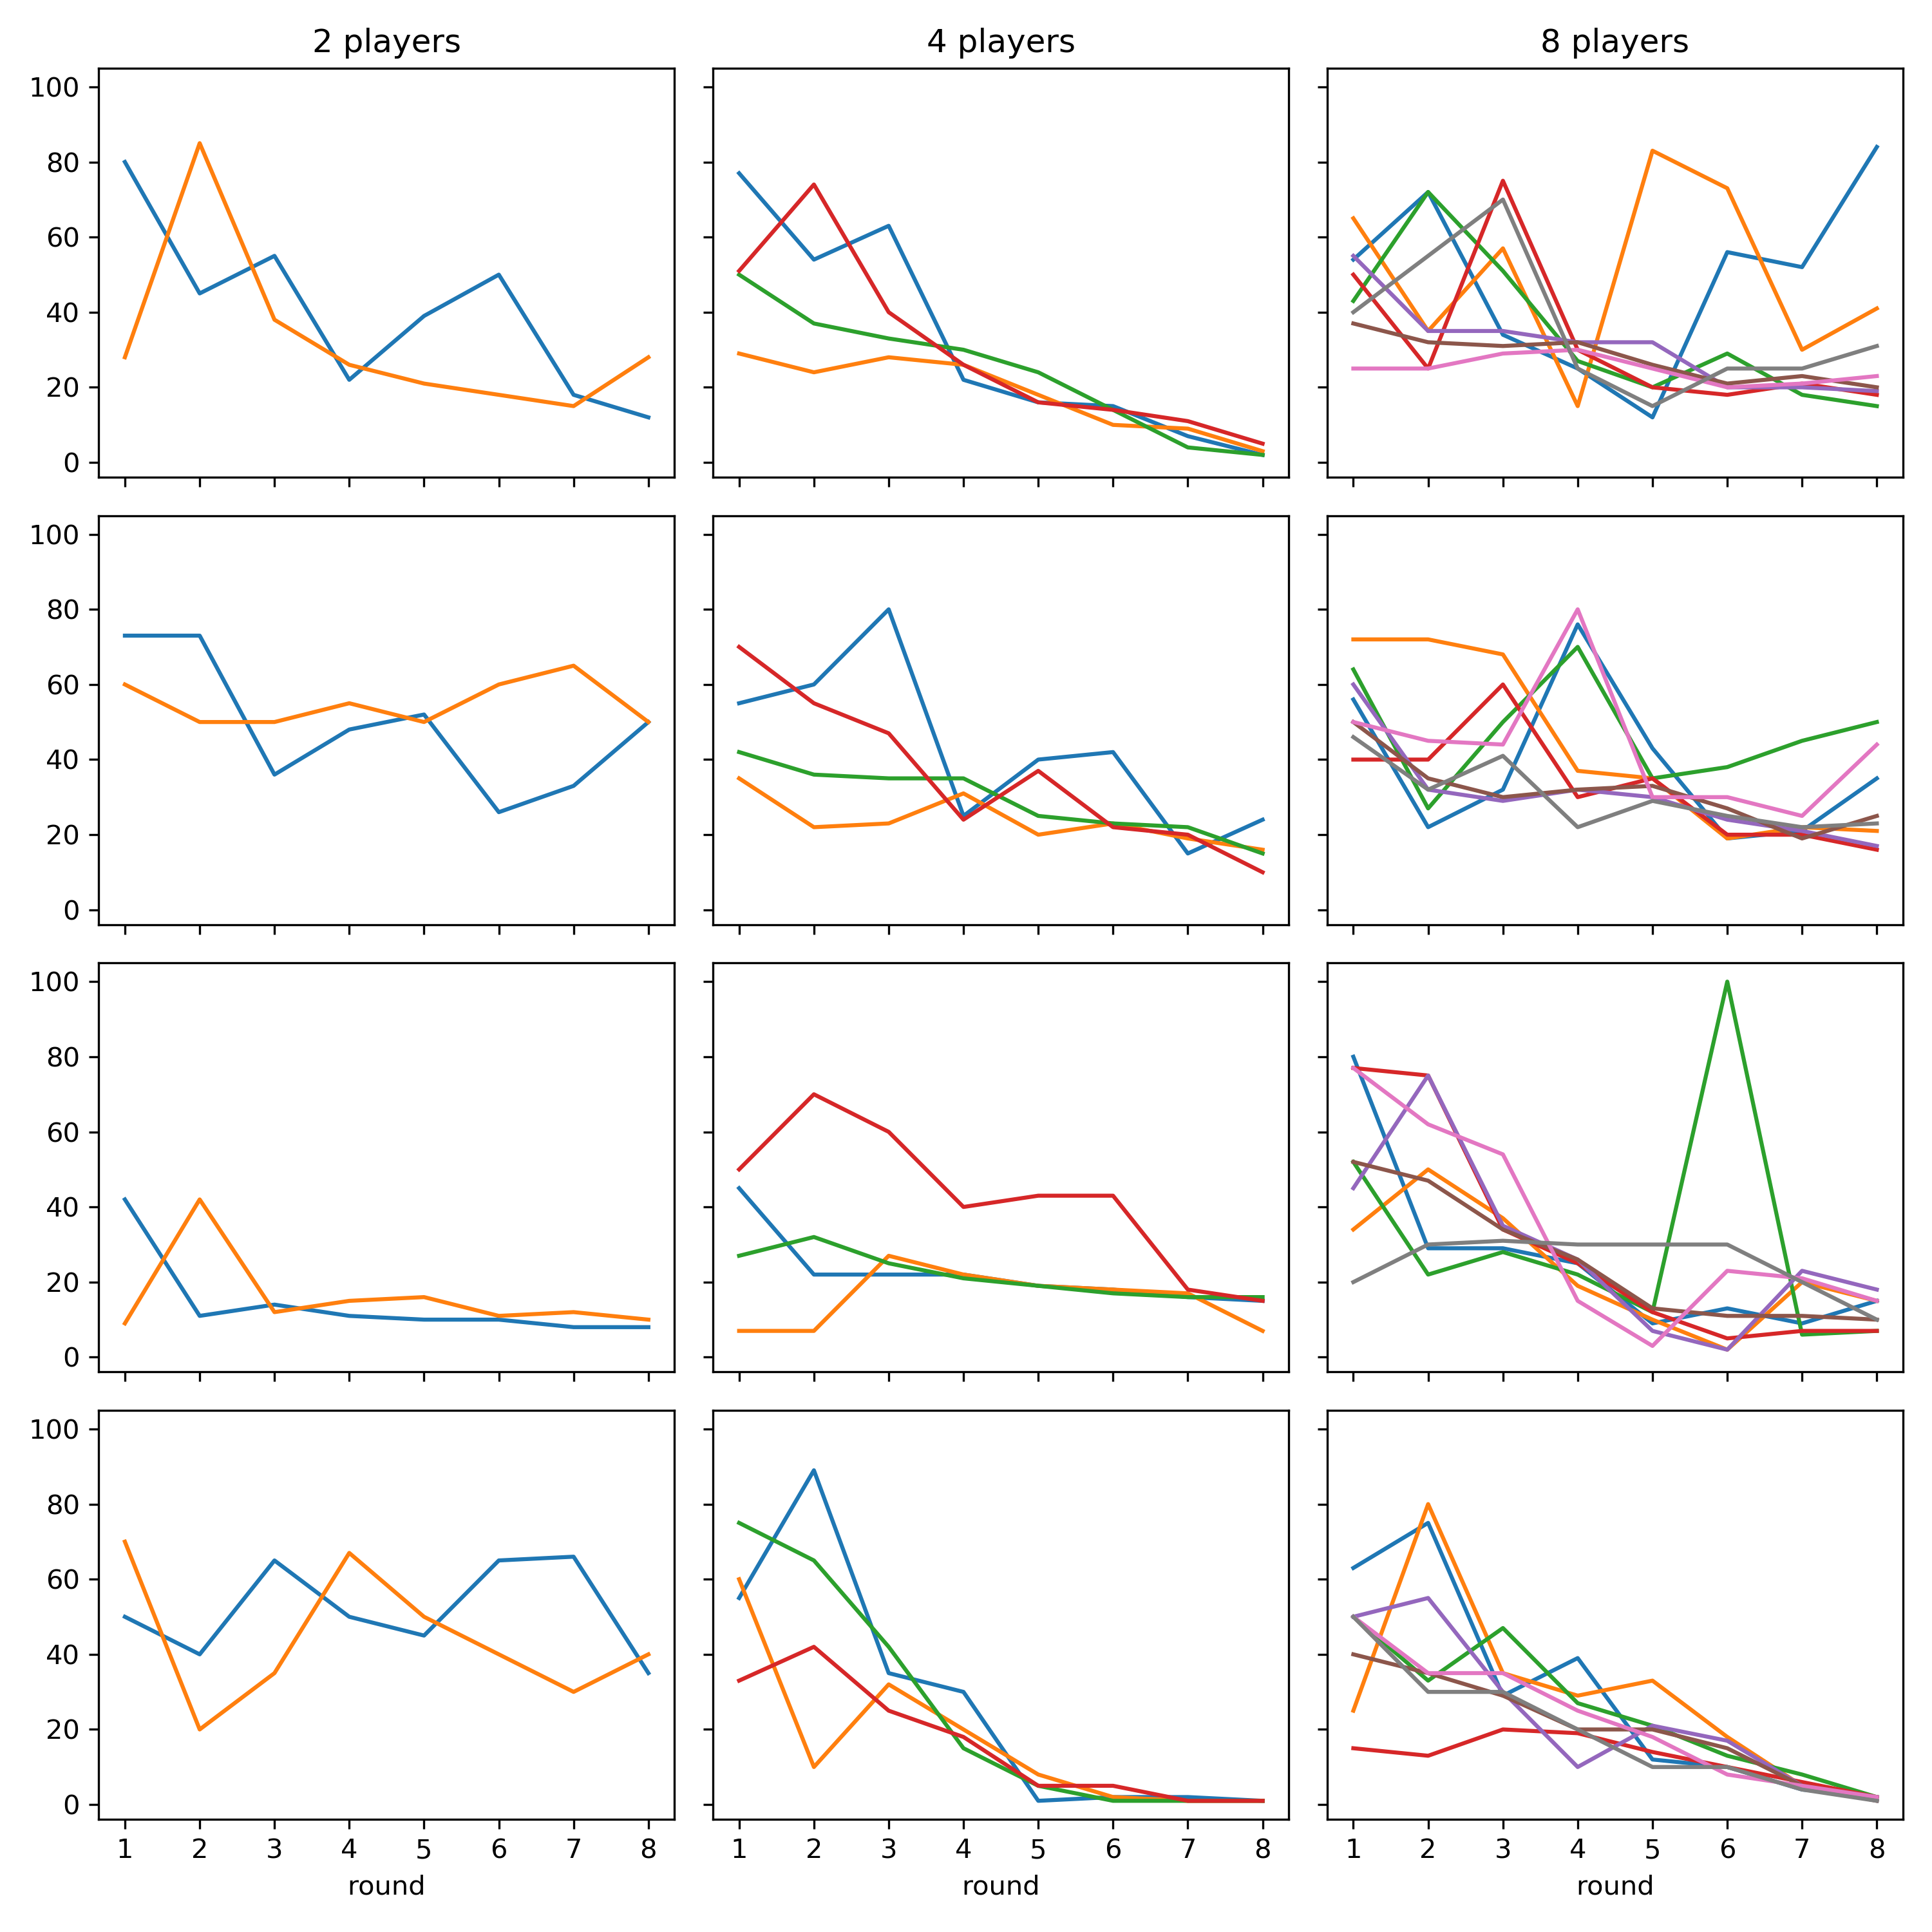
\includegraphics[width=1\textwidth]{../plots/figA6.pdf}\caption{Guess dynamics of player guesses from randomly selected groups.}
%\label{Fig S6}
%\end{figure}
%
%We can illustrate the guess-dynamics in another way as well. 
%Figure \ref{Fig S7} shows the dynamics of guesses round by round in such a way that the previous round n is always shown on the x-axis and the next round $n+1$ is always shown on the y-axis. The diagonal black line corresponds to staying at the same guess in subsequent rounds. Lines connecting the dots in Figure \ref{Fig S7} then indicate the sequence of guesses by the same player, whose comments are shown in the legend. The total bonus earned is shown in parenthesis.

%\begin{figure}
%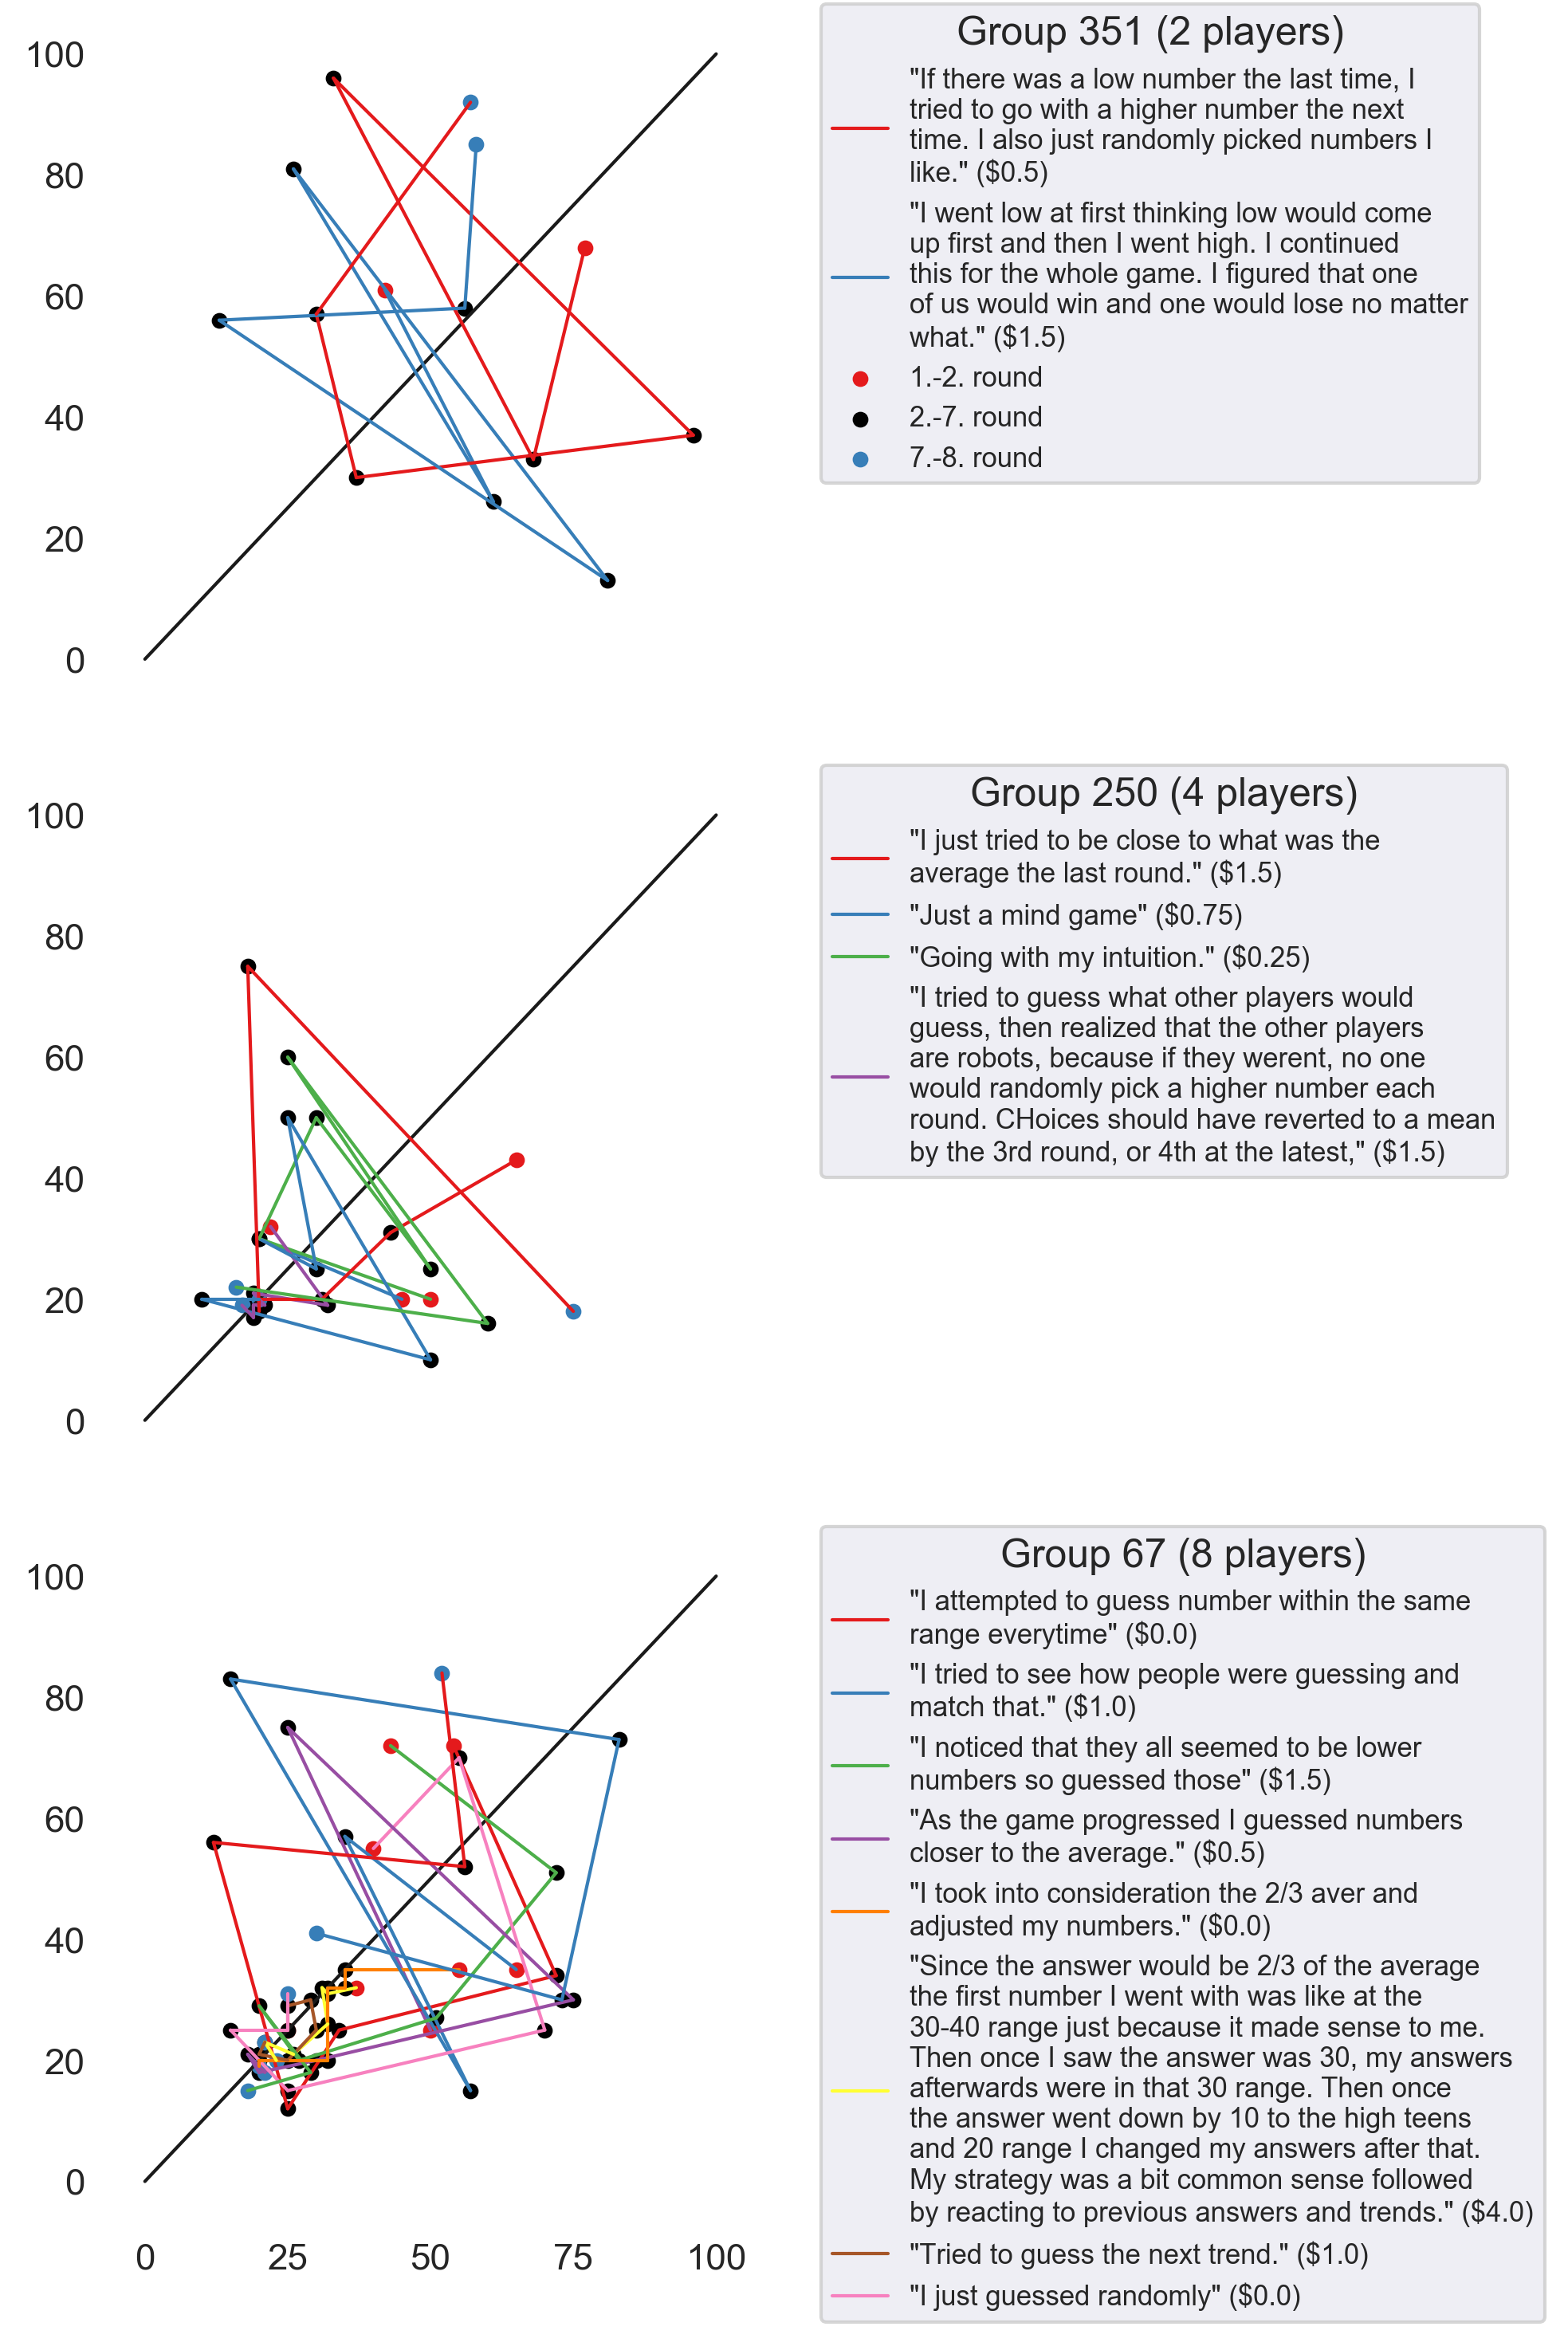
\includegraphics[width=1\textwidth]{../plots/figA7.pdf}\caption{Dynamics of guesses round by round.}
%\label{Fig S7}
%\end{figure}

\section{Learning rates}
\noindent
Based on the observes averages in figure \ref{fig:means} in the main text, we model the averages as a function of rounds and group sizes with a multiple linear regression model containing a quadratic interaction term in the link function, 
\begin{equation}
\mu_{j} =  \alpha_j + \beta_{1j}n + \beta_{2j}n^2 ,
\label{eq:link}
\end{equation}

\noindent
where $\mu_{j}$ is the mean of group $j \in \{2,4,8\}$, $n$ is the round number, $\beta_{1}$ and  $\beta_{2}$ are the slope coefficients for each interaction, and $\alpha$ is a random intercept, which is assumed to be normally distributed with mean $0$ and variance $\sigma^2$. 

To validate the model we plot its standardized residuals against the theoretical quartiles in figure \ref{fig:qq}, which show a very good fit with normally distributed residuals. Tails are obviously not captured all that well, but this is not to be expected. Besides, the linear regression model is quite robust to some degree of deviation from the assumption of normally distributed residuals. In addition, the majority in the middle values are captured near perfectly, hence we cannot reasonably discard the linear regression model.

\begin{figure}[t]
\begin{center}
\includegraphics[width=.5\textwidth]{../plots/qq.pdf}\caption{QQ plot showing normally distributed standardized residuals.}
\label{fig:qq}
\end{center}
\end{figure}

Model outputs of the full model according to equation \eqref{eq:link} are shown in the first column of Table \ref{tab:2}. We see that almost all coefficients are highly significant. The $round^2$ is insignificant, hence the groups of only two players does not exhibit any quadratic form. The interaction between $round^2$ and groups of four is a borderline case, indicating that there might not be any quadratic relationship in this group either. However, the rest of the parameters are highly significant, indicating that (at least) a quadratic term is necessary for the groups of eight players to describe the evolution of the group average over the course of 8 rounds.

\begin{table}[h]
\begin{center}
\begin{tabular}{l c c c }
\hline
 & Full model & First 4 rounds & Final model   \\
\hline
$\beta_{12}$			& $-2.828 \; (.826)^{***}$  & $-6.880 \; (2.717)^{*}$   & $-3.319 \; (.478)^{***}$  \\
$\beta_{22}$			& $.001 \; (.090)$        & $.712 \; (.535)$          &                           \\
$\alpha_{2}$			& $52.821 \; (1.620)^{***}$ & $57.310 \; (2.978)^{***}$ & $53.749 \; (1.310)^{***}$ \\
$\alpha_{4}$			& $52.336 \; (1.689)^{***}$ & $49.209 \; (3.105)^{***}$ & $51.706 \; (1.366)^{***}$ \\
$\alpha_{8}$			& $56.500 \; (1.589)^{***}$ & $51.079 \; (2.920)^{***}$ & $52.690 \; (1.285)^{***}$ \\
$\beta_{14}-\beta_{12}$  & $-3.816 \; (1.193)^{**}$  & $3.665 \; (3.925)$        & $-2.392 \; (.691)^{***}$  \\
$\beta_{18}-\beta_{12}$  & $-6.927 \; (1.157)^{***}$ & $2.148 \; (3.805)$        & $-3.024 \; (.670)^{***}$  \\
$\beta_{24}-\beta_{22}$  & $.245 \; (.129)$          & $-1.212 \; (.773)$        &                           \\
$\beta_{28}-\beta_{22}$  & $.579 \; (.125)^{***}$    & $-1.034 \; (.749)$        &                           \\
\hline
AIC                     & 18344.270                 & 8983.404                  & 8980.375                  \\
BIC                     & 18401.968                 & 9034.171                  & 9015.911                  \\
Log Likelihood          & -9162.135                 & -4481.702                 & -4483.187                 \\
Deviance                & 318129.424                & 134486.544                & 134824.388                \\
Num. obs.               & 2368                      & 1184                      & 1184                      \\
\hline
\multicolumn{4}{l}{\scriptsize{$^{***}p<0.001$, $^{**}p<0.01$, $^*p<0.05$}}
\end{tabular}
\caption{Comparison of regression models. ``Full model'' shows the result of the model in equation \eqref{eq:glm} for all eight rounds. ``First 4 rounds'' shows the result of the same model, but only using the first four rounds, and ``Final model'' shows the result with the first four rounds when the quadratic term is removed. Conversion to table was done with texreg \cite{leifeld2013texreg}.}
\label{tab:2}
\end{center}
\end{table}

The result of the full multiple linear regression model is shown in figure \ref{fig:full}. Groups of two players have a significantly lower learning rate than groups of four and eight players. Learning rates of 4- and 8-player groups are higher, and compare relatively well with previous findings (see figure \ref{fig:means} in the main text). There seems to be a small but significant difference in the learning rates between groups of four and eight in rounds 4-6, which disappears again in the last two rounds. We do not know whether this is due to some artificial last-round effects or a natural leveling off similar to the results in \citet{weber2003learning} as shown in Figure \ref{fig:means} in the main text.

\begin{figure}[h]
\includegraphics[width=1\textwidth]{../plots/fig3_full.pdf}\caption{Learning rates in terms of the decrease in the average guess for groups of 2 (red), 4 (yellow), and 8 (blue) players in the iterated beauty contest on Amazon Mechanical Turk. Crosses show the empirical means, full lines show the result of the multiple linear regression model and shaded areas are the 95\% confidence intervals.}
\label{fig:full}
\end{figure}


However, we only compare the regression model to 4 rounds from other studies, hence a refitted model using only the first 4 rounds is shown in the second column of Table \ref{tab:2}. The fit is still very good with a very similar QQ-plot as in Figure \ref{fig:qq}. In this model the quadratic predictor is insignificant for the first 4 round (ANOVA likelihood ratio test, $p = 0.399$), so that it can be excluded in the final model used in the main text, for which the output is shown in the last column of Table \ref{tab:2}.

\end{document}